\documentclass[10pt,conference]{IEEEtran}

\usepackage{cite}
\usepackage{amsmath}
\usepackage{url}
\usepackage{pdfpages}
\usepackage{soul}
\usepackage{enumitem}
\usepackage{hyperref}
\usepackage{svg}
\usepackage{ulem}
% \usepackage[inkscapearea=page]{svg}
\usepackage{adjustbox}

\hypersetup{
    colorlinks=true,
    linkcolor=blue,
    citecolor=blue,
    filecolor=magenta,      
    urlcolor=blue,
    pdfpagemode=FullScreen,
}

% add page numbers
\pagestyle{plain}


% for comments
\usepackage{color}
\newcommand{\mycomment}[3]{\emph{\textcolor{#2}{#1}: }\textcolor{#2}{#3}}
\newcommand{\todo}[1]{\mycomment{Todo}{red}{#1}}
\newcommand{\sangeetha}[1]{\mycomment{Sangeetha}{magenta}{#1}}
\newcommand{\eric}[1]{\mycomment{Eric}{cyan}{#1}}

% correct bad hyphenation here
\hyphenation{op-tical net-works semi-conduc-tor}

% line spacing: Reference: https://www.overleaf.com/learn/latex/paragraph_formatting#Line_spacing
\renewcommand{\baselinestretch}{1.6}

\begin{document}
% paper title
\title{Perceptron-Based Prefetch Filtering in gem5\\ CS752 Final Project Report}


% author names and affiliations
% use a multiple column layout for up to three different
% affiliations
\author{
\IEEEauthorblockN{Sangeetha Grama Srinivisan}
\IEEEauthorblockA{University of Wisconsin, Madison\\
Email: \texttt{sgsrinivasa2@wisc.edu}}
\and
\IEEEauthorblockN{Eric Brandt}
\IEEEauthorblockA{University of Wisconsin, Madison\\
Email: \texttt{elbrandt@wisc.edu}}}

% make the title area
\maketitle

% As a general rule, do not put math, special symbols or citations
% in the abstract or keywords.
\begin{abstract}
Modern processor speeds far exceed memory access speeds, often allowing 100 instructions to be executed in the same time as one fetch from main memory. Multi-level caches hide much of this latency but when cache misses occur the full access price of main memory must still be paid. Heuristic based `prefetchers' are commonplace today, aiming to reduce compulsory misses by loading the cache with memory that is predicted to be accessed soon. However, a prefetch policy that is too aggressive will load memory that is never used, incurring additional conflict misses and possibly decreasing overall performance. Our project implements a Perceptron-based Prefetch Filter that tunes the aggressiveness of an underlying prefetcher with the goals of increasing cache hit metrics, reducing overall memory bandwidth, reducing power consumption, and increasing overall processor performance. We present background theory, implementation details, measured performance results, related work, and ideas for future study. 
\end{abstract}

\section{Introduction}
Prefetching has been used as an effective strategy to improve processor performance. Many prefetching strategies have been proposed based on spatial or temporal access patterns observed in the program. Until recently, these strategies relied on the designer to conceive, implement, and test novel heuristics, drawing upon his or her on expert experience of observed memory access patterns. These heuristics were coded at design time and could only adapt within their limited range of dynamically tunable parameters built into the design. This is very similar to the original architectural development history of branch predictors. After exhausting the gains of ever-increasingly clever heuristics, the evolution of branch predictor development began to include perceptron-based algorithms. Borrowed from the Artificial Intelligence community, these models `learn' the execution flow at runtime and make intelligent prediction decisions. Now, we are seeing the evolution of prefetcher designs follow a similar course. Machine learning algorithms ranging from simple perceptrons to complex LSTM (Long-Short-Term-Memory) models are leveraged to design and optimise prefetching strategies. One such design uses a perceptron-based prefetch filter\cite{ppf} to enhance Signature Path Prefetching \cite{SPP}, a lookahead prefetcher. In this project we aim to implement this perceptron-based prefetch filter\cite{ppf} in the gem5 \cite{lowepower2020gem5} simulator and evaluate the performance implications of the filtered prefetches on a wide range of workloads. 

Specifically, our paper addresses the following considerations of this topic:
\begin{enumerate}
    \item\textbf{Background}: We discuss relevant existing work, the specific paper that motivated this project, and explain the theory of operation of the Perceptron-based Prefetch Filter
    \item\textbf{Methodology}: We explain the mechanism we implemented within gem5, and discuss the strengths and weaknesses we found in using the existing gem5 infrastructure as a platform for evaluating our prefetch filter.
    \item\textbf{Results}: We explain the details of the benchmarks used and the performance we observed with the prefetch filter.
    \item\textbf{Related Work}: We summarize similar other work related to prefetchers and prefetch filters.
    \item\textbf{Future Work}: We generate ideas and lay out plans for future work that would build upon the foundation our project provides.
\end{enumerate}

\section{Background}
Memory accesses span over multiple cycles. The rate of improvement in memory access speeds compared to the rate of improvement in processor speeds indicates that there is a wide gap known as the Memory Wall \cite{mem-wall}. The increasing gap is shown in the well known Hennessey \& Patterson \cite{hennessey} plot in figure \ref{fig:memwall}. This significant difference in speeds can be mitigated by prefetching memory into the cache to avoid processor stalls while operands are fetched from main memory. The prefetching strategies are continuously being optimised to improve accuracy of prefetching while also maintaining a good coverage, i.e, the prefetcher should be able to eliminate cache misses and all the prefetched memory should be used by the processor. While the former requirement focuses on improving processor performance, the latter requirement helps conserve memory bandwidth and the space availability in the cache. Machine learning algorithms have been used to improve or enhance prefetching, like, offline parameter optimisation for baseline prefetchers or on-line parameter tuning to provide feedback to the prefetcher based on the result of the prefetch, such as the perceptron-based prefetch filter\cite{ppf}. Implementing this filter in gem5 will help in getting a detailed analysis of performance implications on a wide range of program workloads and architectures.  Further, the prefetch filter can be used as a standalone unit with any baseline prefetcher, giving researchers the opportunity to explore the use of this filter with their designs.

\begin{figure}
    \centering
    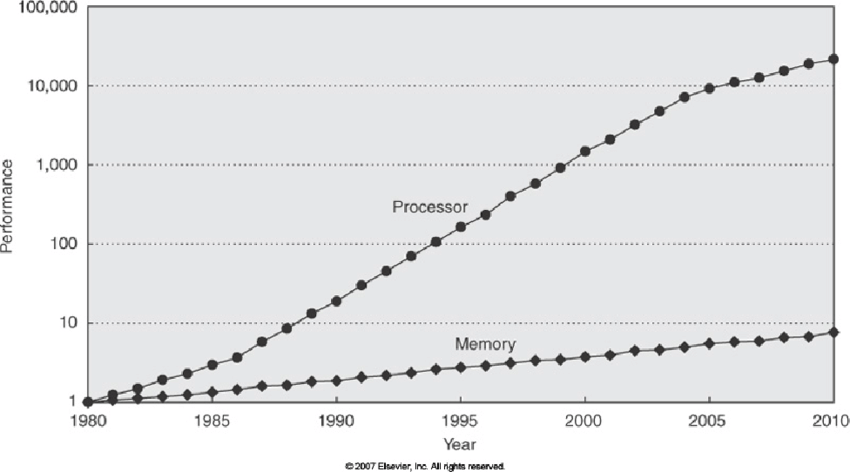
\includegraphics[width=\columnwidth]{Processor-memory-latency-divide-introducing-the-memory-wall-5.png}
    \caption{Graph showing the Memory Wall - difference betweeen the processor performance and memory speeds over time (1980-2010).}
    \label{fig:memwall}
\end{figure}


\section{Methodology}

In this section, we discuss the details of our implementation within gem5, the benchmark development rationale, and the benchmark execution framework we used.

\begin{figure*}
    \centering
    \adjustbox{trim=2cm 4cm 3cm 4cm}{%
        \includesvg[width=2.3\columnwidth]{PPF_Design.svg}
    }
    \caption{Block diagram showing the design of the Perceptron-prefetch filter. Dotted lines indicate data movement for prefetches while solid arrows indicate data accessess as requested by the core.}
    \label{fig:block-ppf}
\end{figure*}

\subsection{Implementation Details}\label{sec:impl}

Gem5 has a wide range of prefetcher implementations including the Access Map Pattern Matching prefetcher\cite{AMPM}, Tagged prefetcher and the Signature Path Prefetcher. All the basic functionality like inserting prefetch requests into a prefetch queue, notifying the MSHR (Miss Status and Handling Register) of completed prefetches, registering listeners to notify on prefetch are implemented in the \texttt{BasePrefetcher} class. The \texttt{QueuedPrefetcher} is derived from the \texttt{BasePrefetcher} and adds support for making a prefetch packet, inserting it into the prefetch queue, and tracking its progress. Every new implementation of a prefetcher in gem5 derives from the \texttt{QueuedPrefetcher}. Every new class that is derived from the \texttt{QueuedPrefetcher} has to implement the virtual function - \texttt{calculatePrefetch}. One such prefetcher, which is derived from the \texttt{QueuedPrefetcher} is the Signature Path prefetcher. There are two implementations in gem5 - \texttt{SignaturePathPrefetcher} and \texttt{SignaturePathPrefetcherV2}. The latter is a revised version of the former based on \cite{sppv2} and is derived from the former. The \texttt{SignaturePathPrefetcherV2} adds a global history register to the earlier implementation. The global history register is an \texttt{AssociativeSet} where each entry is derived from the \texttt{TaggedEntry} class and stores the signature, confidence, offset and the last block information, corresponding to each prefetch suggestion. We use the \texttt{AssociativeSet} and \texttt{TaggedEntry} classes in the implementation of the perceptron-based prefetch filter, which is detailed below. To construct a \texttt{SimObject} and specify parameter values for each of these prefetchers, gem5 has a \texttt{Prefetcher.py} Python wrapper.

As mentioned in \cite{ppf}, we use the baseline prefetcher as the Signature Path Prefetcher for our prefetch filter. Since gem5 has two versions of the Signature Path Prefetcher, we use the newer version, \texttt{SignaturePathPrefetcherV2} as the baseline prefetcher for perceptron-based prefetch filter(PPF). The design of PPF, as shown in Figure \ref{fig:block-ppf} includes a direct-mapped prefetch and reject table with 1024 entries along with weight tables for each feature. The number of weights for each feature is determined by the p-value (confidence statistics) of that feature, as computed in \cite{ppf}. Our implementation of the PPF uses 7 features, which are - Confidence XOR Page address (4096 weights), cache line (4096 weights), page address (4096 weights), base address (4096 weights), confidence (2048 weights), signature XOR delta (1024 weights) and PC XOR delta (128 weights). Delta here refers to the stride for prefetching (as determined by the baseline prefetcher) and signature is a hashed signature generated by the Signature Path Prefetcher. Owing to the difficulty in getting access to the last 3 PCs at the prefetcher level in gem5 and after noticing the low p-value for the feature involving the XOR of the last three PCs, we omit this feature. Note that these features are specific to the baseline prefetcher and will need to change as needed when the baseline prefetcher is different. Each weight in the feature table is a \texttt{SatCounter}, 5 bits wide, which can assume values between -15 and +16. The prefetch and reject tables are implemented as direct-mapped tables using the \texttt{AssociativeSet} implementation in gem5 with LRU as the replacement policy. Each entry of these tables is derived from the \texttt{TaggedEntry} class in gem5 and hence includes methods like \texttt{findEntry}, \texttt{insertEntry} and other methods to keep track of the tag, valid bits and metadata for the LRU replacement policy. The feature tables, prefetch and reject tables are initialised in the constructor of the PPF. Our implementation of the PPF has the provision to accept parameters like threshold from the Python configuration file and default values are specified in the \texttt{Prefetcher.py} Python wrapper file. We also include a flag in the \texttt{SignaturePathPrefetcher} to enable or disable the PPF, which can be controlled from the Python configuration file in gem5. 

\begin{figure*}
    \centering
    \adjustbox{trim=2cm 2cm 2cm 2cm}{%
        \includesvg[width=2.3\columnwidth]{flowchart.svg}
    }
    \caption{A simplified flowchart to depict the change in the workflow with a perceptron based-prefetch filter.}
    \label{fig:flowchart-ppf}
\end{figure*}

Our PPF has 2 public methods as described in its design in \cite{ppf}, which are \texttt{infer} and \texttt{train}. As the name suggests, \texttt{infer} is invoked just before the baseline prefetcher adds a candidate prefetch entry into the prefetch queue in the \texttt{addPrefetch} method of the \texttt{SignaturePathPrefetcher}. Based on the decision from the PPF, it either inserts or rejects the candidate prefetch entry. The input to this method is the prefetch suggestion and all the features mentioned above are extracted from this prefetch suggestion. The last N bits of each feature (where N is the size of the feature table) is used to access the weight in the corresponding feature table. These weights are summed up and compared against the threshold. If the sum is larger than the threshold, the prefetch suggestion is inserted into the prefetch table and the method returns \texttt{true}. In the case where the sum of the weights does not exceed the threshold, it is inserted in the reject table and the method returns \texttt{false}. Note that each entry in the prefetch and reject tables contains all the information necessary to reconstruct the features, which is very helpful for training the corresponding weights. Figure \ref{fig:flowchart-ppf} shows an oversimplified workflow of the prefetcher, with and without the PPF. \texttt{train} is invoked on every access and has the logic to update the weights in the feature table. The information on cache eviction resides in the \texttt{Packet} class but is not directly accessible from the \texttt{SignaturePathPrefetcher}. While we tried to pass this information to the prefetchers through the \texttt{PrefetchInfo} class, we found the changes to be too disruptive and ran into problems with gem5 build. The changes included modifications starting from the \texttt{BasePrefetcher} all the way up to \texttt{SignaturePathPrefetcher} classes. In order to keep other prefetchers functioning along with our PPF and achieve a working version of the PPF, we decided to exclude this feature. Hence, the baseline prefetcher did not have information about cache evictions and we were unable to train weights on eviction in the PPF. As explained in the Results section, we believe this is an unfortunate and significant limitation on the performance of the PPF. On every access to the cache, \texttt{train} is invoked. The PPF checks if this access was a miss and if this access information is found in the reject table by the PPF. If both these checks pass, it implies that the PPF rejected a useful prefetch suggestion and hence, the respective weights need to be updated. A reject implies that the weight sum did not exceed the threshold. Hence, the corresponding weights are incremented by 1. As mentioned previously, since the PPF does not have access to information on eviction from the cache, weights do not get updated for a scenario where the evicted line was not accessed but was prefetched into the cache. We have made a provision in the \texttt{train} method to accept the mode (either access or eviction) and decrement weights for evictions which were prefetched but not accessed. If we were able to get information about eviction in the baseline prefetcher, the only change remaining would be to invoke the PPF \texttt{train} method. 

Alongside these changes, we also modified the \texttt{SignaturePathPrefetcherParams} class and the Python wrapper \texttt{Prefetcher.py} to initialize default values and sizes for PPF parameters like threshold, prefetch and reject table sizes, indexing and replacement policies. In the configuration file that we implemented to run benchmark programs, we initialised a \texttt{SignaturePathPrefetcherV2 SimObject} at the L2Cache level and set the \texttt{enablePPF} flag to \texttt{True} before running the benchmark. The various benchmarks used for evaluating the PPF, along with the results are detailed in the following sections.

\subsection{Benchmark Development}
Evaluating the implementation requires simulation workloads. We selected a variety of workloads that cover a variety of execution patterns. We chose the majority of our workloads from the SPEC2006 benchmark suite \cite{spec2006} primarily because a) the workloads are single threaded, which is easily amenable to gem5 system emulation mode and b) the programs in SPEC2006 are generally simpler and have less dependencies than some later suites, making them ideal for adapting to our time-constrained project. We selected a variety of benchmarks from the suite that we believe have varied data access patterns as well as a combination of integer and floating point computations. The tasks performed by the benchmark programs had to be carefully tuned to yield simulator run times that were agreeable to a reasonable test-anaylze-modify-test cycle required in our development. For this reason, it was not a simple matter of just compiling all benchmarks and letting them run.

In addition to SPEC2006 workloads, we chose two additional benchmarks. First, we included a physics based animation simulation that uses the finite element method to simulate a rubber sheet being stretched an released, based on the methodology described by Sifakis et al. in \cite{sifakis2012}, because such workloads are highly relevant to the authors' primary research interests. Second, we included the ubiquitous and endearing \texttt{daxpy} sample as an homage to CS752 homework assignments.

The relevant primary characteristics of our selected workloads are shown in table \ref{tab:bench}, achieving our goal of simulating a variety expected access patterns and operation types.

\begin{table}[ht]
\centering
\caption{Workload characteristics of benchmarks used}
\label{tab:bench}
\begin{tabular}{c|l|c|c}
\textbf{Benchmark}             & \textbf{Description}                                                      & \textbf{Memory Access} & \textbf{Operation Type} \\ \hline
daxpy                          & \begin{tabular}[c]{@{}l@{}}simple linear\\ algebra test\end{tabular}      & sequential             & floating point          \\
sjeng                          & \begin{tabular}[c]{@{}l@{}}chess game engine\\ AI search\end{tabular}     & random                 & integer                 \\
libquantum                     & \begin{tabular}[c]{@{}l@{}}quantum simulator\\ factorization\end{tabular} & random                 & integer                 \\
povray                         & ray tracing                                                               & random                 & floating point          \\
\multicolumn{1}{l|}{mempinch1} & FEM simulation                                                            & strided                & floating point         
\end{tabular}
\end{table}

The workloads were scripted to be simulated using HTC Condor high throughput cluster. This allowed many combinations of simulations with varying parameters to be tested simultaneously. Specifically, file-driven, parameterized submission scripts were developed to launch a grid of simulations spanning three different processor models (\texttt{SimpleTimingCPU}, \texttt{MinorCPU}, and \texttt{DerivO3CPU}), five benchmarks, and three configurations. 

The three configurations simulated were:
\begin{description}
\item[Baseline] A simple 2-level cache heirarchy with no prefetcher. This includes an 8-way associative L1 cache with a 16kb instruction and 16kb data cache, backed by a 128k 16-way associative L2-cache. Main memory used in this configuration was \texttt{HBM\_1000\_4H\_1x64}. 
\item[SPPv2] The baseline configuration enhanced with the gem5 Signature Path Prefetcher v2 attched to the L2 cache, configured with to prefetch on cache misses. (We encountered an issue in gem5 which prevented us from configuring the prefetcher to activate on cache accesses in addition to cache misses. The details of this configuration difficulty seem to be outside of the scope of this PPF implementation).
\item[SPPv2+PPF] The SPPv2 configuration embellished with our Perceptron Prefetch Filter, implemented as described above.
\end{description}

Because the Condor submission script was written to be parameterized, future work that expands the number of configurations, for example testing with different hyperparameters for the PPF, will be a trivial modification of the submission script. A Python analysis script was written to parse statistics from the grid of \texttt{m5out/stats.txt} files, similarly making future expansion of testing scope relatively trivial. The Condor scripts, submission files, and analysis scripts can be found in the Github repository linked in Errata, section \ref{sec:errata}, at the end of this paper.

\subsection{Results}
The results of our work can be evaluated from both a quantitative and qualitative viewpoint. 

\subsubsection{Quantitative Results}

The quantitative results are best viewed as statistics extracted from the \texttt{m5out/stats.txt} files from each of the simulations that were executed. Prior to the Condor simulations finishing, we identified a variety of statistics that we felt would be relevant to evaluating the performance of our prefetch filter. These statistics included:
\begin{enumerate}
    \item Instructions per Cycle - the ultimate measure of workload performance: how many instructions the processor was able to execute per clock cycle of runtime.
    \item Prefetches Issued - the number of prefetches issued. In theory if the filter is doing its job properly, this number should decrease with the filter enabled, while not resulting in a meaningful drop in cache hit ratio.
    \item Useful Prefetches  - the number of prefetches that were eventually accessed by the program before being evicted. The ratio of this value to prefetches issued should increase if our filter is effective.
    \item Unused Prefetches  - the number of prefetches that were loaded into cache, but never accessed by the program before being evicted. Our filter should cause this metric to decrease.
    \item Total memory bandwidth  - the total amount of data that traveled over the memory bus between DRAM and L2 cache. Effective filtering should cause this value to decrease, without incurring a loss of performance. This is also a good proxy for power consumption, because retrieving data from DRAM is one of the highest power consuming activities within a computer. 
\end{enumerate}

After extracting the relevant statistics and discussing the results, we realized that many of the statistics above have a strong correlation with each other, essentially confirming the validity of the results and reinforcing our confidence in the effect of the configuration changes. For example Unused Prefetches resulted in nearly identical information as the ratio Useful Prefetches / Prefetches Issued, in this case having a near perfect negative correlation. For that reason, only a subset of the statistics are presented here, to avoid duplicating very similar data.

The most coarse-grained indication of performance difference is in the Instructions per Cycle (IPC) achieved in each configuration for the \texttt{DerivO3CPU} shown in table \ref{tab:ipc} (higher is better). This  table shows that certainly having a prefetcher helps (SPPv2 vs. Baseline), while our implementation of the prefetch filter yielded mixed results. In all cases, the difference in performance between SPPv2 and SPPv2-PPF was very minor, the reason for which is explained in the qualitative discussion about the results.
\begin{table}[ht]
\caption{Instructions per cycle for each benchmark using DerivO3CPU (higher is better).}
\centering
\begin{tabular}{l|rrr}
Benchmark &  Baseline &     SPPv2 &  SPPv2-PPF \\
\hline
daxpy      &  0.6778 &  \textbf{0.8375} &   0.8297 \\
libquantum &  1.8765 &  1.8769 &   \textbf{1.8771} \\
mempinch1  &  0.9942 &  0.9945 &   \textbf{0.9945} \\
povray     &  1.0498 &  1.0497 &        N/A \\
sjeng      &  0.3293 &  \textbf{0.3880} &   0.3879 \\
\end{tabular}
\label{tab:ipc}
\end{table}

Two statistics that are more fine-grained are the number of prefetches issued and the number of prefetches that went unused, shown in Table \ref{tab:pref}, again for \texttt{DerivO3CPU}. In this case we can again see that the filter is indeed, generally, reducing the number of prefetches that are issued, and more importantly, reducing the number of prefetches that go unused, as those are wasted memory bandwidth.  Two interesting observations can be made by closely examining this table: First, consider the \texttt{daxpy} benchmark program. In the case of this algorithm, only the true `daxpy' loop is included in the statistics, by use of the \texttt{m5ops} magic functions. In this tight loop, the prefetcher is able to perfectly predict the sequential memory access, and every prefetch that is issued is used. Note that in the PPF configuration, some of the prefetch requests are erroneously rejected, and this is almost certainly the reason that Table \ref{tab:ipc} showed a higher IPC for the SPPv2 configuration over the SPPv2-PPF configuration. It would appear that in very regular sequential access patterns, the prefetch filter has the opportunity to hurt near perfect prefetching performance.

A second observation in this table is that the \texttt{sjeng} benchmark shows that even though SPPv2-PPF issued less prefetches, it actually had more of those prefetches that it issued go unused. This is initially counter-intuitive, because, being a `filter', the PPF can only veto the request to perform prefetches, not suggest new prefetches of its own. However, there are reasonable explanations for these statistics. It is important to remind ourselves that these statistics are only about prefetches to the cache. Certainly all memory that was requested by the application was eventually retrieved into the cache, but in the SPPv2-PPF case, obviously more of those requests were serviced by (potentially stalling) loads rather than proactively by the prefetcher. So, it is certainly possible that even though the SPPv2-PPF caused the prefetcher to do less work, the work that it did do was of lower quality (more prefetches went unused). This explanation would also predict that the overall IPC of this benchmark would be lower with the SPPv2-PPF configuration, which is reassuring to see, is indeed the case in Table \ref{tab:ipc}.

\begin{table}[ht]
\caption{Total number of prefetches issued versus number of prefetches unused (lower unused is better).}
\centering
\begin{tabular}{l|rr|rr}
&  \multicolumn{2}{c|}{SPPv2} & \multicolumn{2}{c}{SPPv2-PPF} \\
Benchmark &  Issued &      Unused &  Issued & Unused \\
\hline
daxpy      &     1,310 &   0 &     1,281  & 1\\
libquantum &     1,709 & 113 &     1,655 & \textbf{106} \\
mempinch1  &     3,117 & 460 &    3,062 & \textbf{434} \\
povray     &   370,650 & 83,335 &      N/A & N/A \\
sjeng      & 2,719,591 & \textbf{5,120} & 2,719,167 & 5,131 \\
\end{tabular}
\label{tab:pref}
\end{table}

A final quantitative result to discuss is the total memory bandwidth utilized by each benchmark, shown in Table \ref{tab:mem}. This table shows the number of bytes traveling across the DRAM bus. In this table, we see exactly what we would expect: Because the filter is reducing the number of prefetch requests, we see a decrease in total memory transferred. The only way we would not see a decrease would be if a) the prefetcher issed no prefetch requests at all, or if b) the filter approved all prefetch requests. Any other scenario necessarily requires the SPPv2-PPF statistics to show less memory traffic on the bus. In a perfect case, the memory traffic that is reduced is made up entirely of prefetch requests that go unused, but this is too optimistic of a view, as earlier statistics have proven. We also note that this statistic has a very useful additional interpretation as being a proxy for one aspect of power consumption. As is well known, retrieving data from main memory requires a relatively high amount of power compared to other execution related operations. Therefore, reduced memory bandwidth utilization also should correspond to reduced power consumption. To determine if the overall energy cost to run the program is less, one would have to incorporate many other factors, including total number of cycles for execution, so by itself this metric is not a pure indicator of absolute efficiency, but is a relevant component.

\begin{table}[ht]
\caption{Total memory bandwidth used from DRAM to L2 Cache, in bytes. (Lower is better)}
\centering
\begin{tabular}{l|rrr}
 Benchmark &  Baseline &        SPPv2 &    SPPv2-PPF \\
\hline
daxpy      &       N/A &  206,117,582 &  \textbf{200,628,483} \\
libquantum &       N/A &     230,557 &     \textbf{223,376} \\
mempinch1  &       N/A &     706,978 &     \textbf{690,513} \\
povray     &       N/A &   12,118,251 &        N/A \\
sjeng      &       N/A &  124,682,642 &  \textbf{124,656,298} \\
\end{tabular}
\label{tab:mem}
\end{table}

\subsubsection{Qualitative Results}

It is no secret that the quantitative differences in our results between SPPv2 and SPPv2-PPF are quite small. Therefore, it is important to discuss the qualitative results, and the reasons that the impact of the PPF was smaller than expected (and indeed, smaller than achieved by Bhatia et al. in their original work \cite{ppf}). We believe the primary reason for the small impact is the inability within gem5 to use cache eviction as a trigger to tune the perceptron weights. This architectural limitation is discussed thoroughly in Section \ref{sec:impl} Implementation, but restated here for emphasis. The crucial observation is that good information about whether a prefetch was worthwhile is only available when it is known if the prefetched memory was actually used. While this information is available in the gem5 Cache objects, it was not readily available in the Prefetcher object to be able to be passed to our prefetch filter. This design could certainly be adapted given more time to implement, but within the constraints of this project this was not a feasible modification to the gem5 source code. Without this information, good training information for training the perceptron weights was not available, and hence the perceptron probably did not achieve high accuracy as a binary classifier of good versus bad prefetch requests.  Based on weight-debugging information we logged during development, we hypothesize that it `learned' to be very conservative when rejecting requests, and when it did reject the requests, was often times not very confident in its decision. 

Another hypothesis we made at the outset was that the \texttt{SimpleTimingCPU} would gain the most by use of the SPPv2-PPF configuration. Our intuition was that with such a simple pipeline that is required to stall at memory accesses, that having the cache more often already populated by prefetches, the impact on overall performance would be greater. We felt that the more advanced pipelines of \texttt{MinorCPU} and \texttt{DerivO3CPU} would benefit less because they had other mechanisms available to hide memory latency (e.g. multiple functional units, ROB for out of order execution). However, our simulation data showed a mostly even effect of the PPF across all three CPUs. Perhaps the \texttt{SimpleTimingCPU} is so limited by its simple pipeline that no single isolated improvement is sufficient to deliver significant performance gains. Furthermore, we found almost no statistical difference in PPF effect between \texttt{MinorCPU} and \texttt{DerivO3CPU}, again, likely due to the limited impact of the PPF in general due to the implementation limitations discussed above.

\section{Related Work}

We can broadly classify prefetching mechanisms into 2 categories - Spatial prefetching and Look-ahead prefetching. The former does not take into account the order of accesses while the latter does. One such spatial prefetcher is the AMPM\cite{AMPM}, which proposes Access Map Pattern Matching to generate and issue prefetches. As the name suggests, the mechanism uses pattern matching to identify memory access pattern and generate prefetch requests. In order to do so, the main memory is partitioned into many zones, and 'hot-zones' are identified based on the latest memory accesses issued from the CPU. A map is used to store the memory accesses in these zones, with the help of which a pattern, which is nothing but the stride, is determined. For each line in the zone, the map uses a 2 bit value to track the accesses: Init/Prefetch/Access/Success. These states along with the identified access pattern of that zone are used to issue prefetches.  

Pugsley et al. present a prefetching technique known as Sandbox Prefetching\cite{sandbox}, which is another spatial prefetcher. The design first uses global pattern confirmation of the cache accesses using a Bloom filter and once the pattern is confirmed, can immediately start prefetching addresses using the confirmed pattern. The sandbox is used to prevent unwanted memory accesses and conserve memory bandwidth and pages available in the cache. Within the sandbox, the prefetcher matches the program’s cache access patterns with one of the candidate patterns (each with a different offset). The candidate pattern for which most of the memory accesses match is treated as the confirmed pattern and prefetches are issued using this pattern. While the design reduces the prefetch aggressiveness and uses spatial locality, it does not take into account the program order for prefetching memory.

Signature Path Prefetching \cite{SPP} (SPP) is a type of a Look-ahead prefetcher where program order is taken into account. SPP is designed to not only predict the memory location accessed but also the order of the access within a given page. The method predicts the future memory access patterns without requiring inputs from the PC or the branch predictor. The design has 3 components - Signature table, Pattern table and the Prefetch engine. The signature table stores the physical page numbers, the previously accessed block in that page along with a hash of the previous access patterns to that page, compressed as a signature. The pattern table, indexed using this signature, is used to store future stride access patterns and the confidence for each of the prospective prefetch patterns. The pattern table is indexed by the signature, unlike the signature table which is indexed using the physical page number since multiple pages can have the same memory access pattern. The prefetch engine issues the prefetch pattern which has a confidence greater than a threshold (known as filtering) and also performs lookahead by using a lookahead signature. This lookahead signature is generated from the old signature and used to access the pattern table again to look further ahead and find more prefetch candidates, repeating the prefetching process. Though the design is simple and performs better than spatial prefetchers like AMPM\cite{AMPM}, the effectiveness of the design is dependent on the threshold used to determine if a prefetch pattern with a certain confidence value can be issued.

In search of new techniques to improve the performance of prefetchers, Peled et al. \cite{semantic-locality} proposed a novel idea where the program is used to determine `semantic locality', irrespective of the machine's physical memory alignment. The method is designed based on the observation that the program issues memory access instructions and hence, analysing the program should give more information when compared to the physical memory layout. This extracted information is then used to design and direct the decisions of a context-based prefetcher. Using a particular flavor of reinforcement learning known as the \textit{contextual bandits},  prefetch requests are evaluated, assigning a positive or negative reward. However, this technique is dependent on the semantic analysis and requires support from the compiler. 

The same year as Peled's proposal, Shevgoor et al. proposed a Variable Length Delta Prefetcher (VLDP) \cite{VLDP} that purely uses heuristics on accumulated history to tune the prefetch strategy rather than relying on compiler direction or machine learning. The VLDP algorithm watches successive cache line misses in each physical page, stores the deltas of those misses in a history table, and then uses that table to predict the cache line misses in new pages. As each successive miss in a page occurs, the `delta history' for that page grows longer. The first entries of the that longer history can be matched to other pages with shorter histories, and thus used to predict the next accesses within those pages. This is an example of a global history approach, and achieved performance exceeding both other global history approaches and PC-counter based approaches.

Finally, the prefetch strategy of interest to our work is the recent design by Bhatia et al \cite{ppf}. His group proposed a simpler method of using a perceptron-based prefetching filter to control the aggressiveness of prefetchers. The method is implemented using SPP\cite{SPP} as the baseline prefetcher. Since in SPP, the threshold for confidence is used to determine whether a prefetch needs to be issued, using a perceptron to make this decision helps in 2 aspects. First, it provides a generalisation of the process used in SPP to decide to issue a prefetch and secondly, it helps to decide which level of memory to prefetch into based on the output of the perceptron. The SPP method in \cite{SPP} reserved a part of the L2 cache for prefetching while the perceptron-based prefetching filter allows prefetching to be done either to L2 or the next cache level. The filter acts as a check to control the aggressiveness of the prefetcher by maintaining 3 tables - weight table, prefetch table and a reject table. The weight table maintains the weight for each feature (input to the perceptron) and is used to compute the weighted sum of the features - the confidence level of the prefetch, which is then compared against a threshold. The prefetches that have a confidence level higher than the threshold are stored in the prefetch table, while those that do not are stored in the reject table, both of which are used to tune the weights in the perceptron. Training is done when an address from the memory request is found in either of the tables, indicating a correct or a misprediction following which the weights are updated accordingly. This design uses the perceptron-based prefetch filter as a stand-alone module that can be used with any type of baseline prefetcher, and thus, can enhance any existing prefetcher. 

\section{Conclusion}
In this section, we outline some improvements that can be made to our project and summarize our implementation of the perceptron-based prefetch filter. 

\subsection{Future Work}
Our implementation of the perceptron-based prefetch filter is not similar in performance to the design in the reference paper\cite{ppf}. We believe this difference can be attributed to the deviations we were forced to take from the paper, owing to gem5 design and implementation difficulties. We also faced some intermittent undesired behavior within gem5, that we were not able to reproduce consistently, but hindered debugging in some configurations like \texttt{prefetch\_on\_access=True}. In the time allotted for this project, we were able to implement an albeit modified, working version of the perceptron-based prefetch filter. A first step towards extending this work would be to minimize the implementation deviations from the reference paper\cite{ppf}. Out of the two deviations that we had to take, training the perceptron weights on cache eviction is one major factor, which when implemented, should drastically improve the performance of the filter. The other one, which involves the last 3 program counters information as a new feature, can be included once the training on eviction logic is complete. Since we already see some performance improvement with the existing implementation, closing the gap on these two deviations will definitely give a boost to this improvement. Further, some effort can be invested into tuning the threshold for the perceptron-based prefetch filter for various benchmarks. With our flexible and parameterised benchmark scripts and access to the threshold parameter from the gem5 config file, this task becomes a simple parameter search involving many runs and a similar result analysis as we have done above for each threshold value. 

\subsection{Summary}
Through this project, we aimed to get a working perceptron-based prefetch filter implementation in gem5 and more importantly, learn more about prefetchers and caches through this process. While the in-class homework definitely made us comfortable with running experiments using gem5, diving into this huge codebase with so many different components was an exciting experience. The code in gem5, at least the cache and prefetcher modules, are well organised and clearly differentiated. However, it took significant effort to read through the code and understand the dependencies and isolate the files relevant to our implementation. With the help of debug flags and multiple runs of a simplified daxpy benchmark, we were able to debug our implementation of the perceptron-based prefetch filter and get it working. Though we had to make some changes in the design, we were able to successfully implement most of the functionality and run benchmarks in the time alloted for this project. We have also ensured that our design of the filter is suitable to add more functionality without requiring many changes. Our scripts used to run benchmarks can also be used to run any benchmark to test any other features in gem5 with minimal changes. While the authors of the reference paper\cite{ppf} use a much simpler looking simulator known as ChampSim\cite{champsim}, we have been successful in bringing this idea to a much bigger simulator like gem5. With the various prefetcher implementations in gem5, we hope that this work on the perceptron-based prefetch filter will be continued and the filter can enhance the performance of the baseline prefetchers, serving its purpose. 

Below, we list the original milestones contained in our project proposal. For each, we have commented in \textit{italics} on the status of the item at project submission. We have overstriked milestones that we were able to successfully complete.
\begin{itemize}
\item\textbf{Milestone 1}: Tasks that we plan to complete before the progress report deadline:
  \begin{enumerate}
    \item \sout{Survey the prefetch mechanisms that exist within Gem5 today. We will gain understanding of the implementation of cache prefetch mechanisms by studying of the files in \texttt{src/mem/cache/prefetch}, with careful attention paid to \texttt{signature\_path\_v2.cc}, and the inheritance hierarchy of classes within that folder.} \textit{Completed.}
    \item \sout{Continue a more comprehensive literature review of current cache prefetch strategies to better understand the lineage of the Preceptron Prefetch design. Particular attention will be given to studying the design of Signature Path Prefetching, as this is the groundwork on which Perceptron-Based Prefetch Filtering is built.} \textit{Completed.}
    \item \sout{Develop/curate a set of benchmarks and statistics on which to evaluate various prefetch strategies. This includes development of scripts to run the benchmarks in Gem5 as well as analyze the generated statistics.} \textit{We initially ran into some difficulties here with getting access to the SPEC2006 benchmark which we resolved later. The benchmarks as downloaded did not build automatically via the included Perl scripts, so individual benchmarks were hand selected, and adapted as necessary to build in gcc 9.5 instead of the original (now outdated) gcc 4.3.}
    \item \sout{Create a new trivial-capability C++ prefetch object within Gem5, likely derived from \texttt{Prefetcher::Base} or \texttt{Prefetcher::Queued}, with associated Python wrappers, exposing settings that allow the prefetcher to be tuned via Gem5 Python system definition scripts.} \textit{Completed.}
    \item \sout{Test the framework of the new trivial prefetcher by ensuring our benchmarks can be executed on simulation systems defined to use this prefetcher within the memory heirarchy.} \textit{Completed.}
    \item \sout{Prepare and submit a mid-project progress report by the November 13 deadline.} \textit{Completed.}
  \end{enumerate}
\item\textbf{Milestone 2}: Tasks that we plan to complete before the Lightning Talk deadline
  \begin{enumerate}
      \item  \sout{Implement the Perceptron Prefetcher described in Bhatia et al. by modifying the trivial prefetcher created in Milestone 1.} \textit{Completed.}
      \item \sout{Develop test programs for execution in Gem5 that are both simple, and specifically engineered to test the correctness of the implementation of the Perceptron Prefetcher.} \textit{We used a simplified daxpy program for debugging, because the memory access patterns of daxpy were simple and well understood.}
      \item \sout{Benchmark our implementation to test both for correctness of implementation, and for performance using the scripts developed in Milestone 1.} \textit{We resolved the problem with SPEC2006 and used some workloads from the SPEC2006 benchmark and some physics-based simulation benchmarks.}
      \item \sout{Compare performance of key statistics with other prefetch designs that already exist in Gem5.} \textit{Completed. Compared with SPPv2}.
      \item \sout{Prepare a `Lightning-talk' to evangelize the work and results involved in this project by December 2.} \textit{Completed.}
      \item \sout{Write a `research paper'-quality report of our work and the results we measure by December 15.} \textit{Completed.}
  \end{enumerate} 
\item\textbf{Stretch Milestones}: Tasks that we hope to complete, but may be too large to fully complete within the time constraints of the project.
  \begin{enumerate}
      \item Increase the number of `tunable' settings exposed by our Perceptron Prefetcher, to allow for more experimentation. \textit{A reasonable restatement of this stretch goal would be to open up the architecture of gem5 cache object model to supply additional critical information about cache line usage and eviction to the prefetch layer. This is a more significant undertaking that will take more time.}
      \item Perform a more exhaustive evaluation of the effect of the available settings of our prefetcher with various different cache configurations in simulated systems. \textit{This is a reasonable next step after adapting gem5 to obtain access to information that will allow more effective training of the perceptron weights}.
      \item Test different workloads to try to discern the particular conditions and code characteristics that favor the Perceptron Prefetcher as compared to other strategies. It may be interesting to run different prefetch strategies on physics-based-animation/simulation workloads, to compare prefetch performance in generalized benchmarks (e.g. SPEC CPU) with the numerical, highly-regular access patterns of this type of domain-specific code. \textit{We purposefully and carefully selected workloads that had a variety of different memory access patterns, and used a variety of different functional units. Due to the implementation difficulties noted in the report, it was difficult to discern any behavioral differences due to these workload differences, with the notable exception of daxpy.}
      \item Evaluate our implemented prefetch filter on prefetch strategies other than Signature Prefetch, to ascertain the transferability of a prefetch filter to other prefetch strategies. \textit{This remains an  an interesting idea to pursue, but primarily of academic nature. As a practical matter, it only seems worth the time investment to use the PPF on the state-of-the-art prefetcher. We are not sure of rationale for attempting to use it on any sub-par prefetchers.}
      \item \sout{Propose ways to further improve the design of the Perceptron Prefetcher, or at least define roadmaps for future research.} \textit{Interestingly, the original authors of the design have drafted a followup paper that suggests improvements to the design of Signature Path Prefetcher that work synergistically with the Perceptron Prefetch Filter design \cite{Bhatia2019EnhancingSP}. It would be interesting to apply these changes to our implementation and again evaluate the effect.}
  \end{enumerate}
\end{itemize}

\section{Errata} \label{sec:errata}
\subsection{Contribution Statements}
% \begin{description}
Throughout this project, we have been able to get a good and equal split of work between the two of us. While the split has been detailed below, we were both involved in helping/debugging each other's work. 
\begin{itemize}
    \item Eric Brandt: The work of this project can be categorized in computing terms as `cooperative multitasking.' After topic selection and proposal acceptance, I was primarily responsible for the tasks of finding, preparing, and tuning benchmarks with characteristics relevant to what we hoped to show in our results, with Sangeetha offering valuable input. I set up the Condor build of our gem5 fork and prepared the parameterized submissions scripts. I provided support as needed to the gem5 development, including running gem5 in the gcc debugger to help track down implementation issues. I prepared the Python script to extract statistics from the \texttt{m5out} files, and discussed with Sangeetha how best to present our results. Responsibility was shared in preparation of the progress report, lightning talk, presentation, and final report. The elusive \texttt{prefetch\_on\_access} issue consumed much of our time jointly.
    \item Sangeetha Grama Srinivasan: While Eric worked on setting up the benchmarks and the condor scripts, preparing the lightning talk and scripts to tabulate results etc., I worked on the perceptron filter implementation in gem5 - which involved understanding and exploring the code, implementing the functionality of the perceptron and debugging the perceptron filter and the \texttt{prefetch\_on\_access} issue with Eric's help. I also contributed to the reports, lightning talk, and presentation along with Eric.
\end{itemize}
% \end{description}

\subsection{Project Code \& Tools}
The source code to our implementation of a Perceptron Prefetch Filter for gem5 can be found at \mbox{\url{https://github.com/sanggs/gem5/tree/ppf}}.

The source code to the benchmarks, test scripts, Condor submission scripts, analysis scripts, and other related files can be found at \mbox{\url{https://github.com/elbrandt/CS752\_Proj}}.

This research was performed using the compute resources and assistance of the UW-Madison Center For High Throughput Computing (CHTC) in the Department of Computer Sciences. The CHTC is supported by UW-Madison, the Advanced Computing Initiative, the Wisconsin Alumni Research Foundation, the Wisconsin Institutes for Discovery, and the National Science Foundation, and is an active member of the Open Science Grid, which is supported by the National Science Foundation and the U.S. Department of Energy's Office of Science.


\clearpage

\newpage
% references section
\bibliographystyle{IEEEtran}
\bibliography{IEEEabrv,ref_final}
% \newpage

\clearpage
% \includepdf[pages={1-3}]{BrandtSrinivisan_CS752ProjectProgress-watermarked.pdf}

\includepdf[pages={1}]{cs752-projectChecklists-finalReport.pdf}

% that's all folks
\end{document}

